% THIS IS SIGPROC-SP.TEX - VERSION 3.1
% WORKS WITH V3.2SP OF ACM_PROC_ARTICLE-SP.CLS
% APRIL 2009
%
% It is an example file showing how to use the 'acm_proc_article-sp.cls' V3.2SP
% LaTeX2e document class file for Conference Proceedings submissions.
% ----------------------------------------------------------------------------------------------------------------
% This .tex file (and associated .cls V3.2SP) *DOES NOT* produce:
%       1) The Permission Statement
%       2) The Conference (location) Info information
%       3) The Copyright Line with ACM data
%       4) Page numbering
% ---------------------------------------------------------------------------------------------------------------
% It is an example which *does* use the .bib file (from which the .bbl file
% is produced).
% REMEMBER HOWEVER: After having produced the .bbl file,
% and prior to final submission,
% you need to 'insert'  your .bbl file into your source .tex file so as to provide
% ONE 'self-contained' source file.
%
% Questions regarding SIGS should be sent to
% Adrienne Griscti ---> griscti@acm.org
%
% Questions/suggestions regarding the guidelines, .tex and .cls files, etc. to
% Gerald Murray ---> murray@hq.acm.org
%
% For tracking purposes - this is V3.1SP - APRIL 2009

\documentclass{acm_proc_article-sp}

\usepackage[slovene]{babel}
\usepackage[utf8]{inputenc}
\usepackage{url}
\usepackage{graphicx}
\usepackage{float}
\graphicspath{ {images/} }
\usepackage[usenames, dvipsnames]{color}

\begin{document}

\title{Priporočanje športnega treninga na podlagi prejšnjih aktivnosti}
%
% You need the command \numberofauthors to handle the 'placement
% and alignment' of the authors beneath the title.
%
% For aesthetic reasons, we recommend 'three authors at a time'
% i.e. three 'name/affiliation blocks' be placed beneath the title.
%
% NOTE: You are NOT restricted in how many 'rows' of
% "name/affiliations" may appear. We just ask that you restrict
% the number of 'columns' to three.
%
% Because of the available 'opening page real-estate'
% we ask you to refrain from putting more than six authors
% (two rows with three columns) beneath the article title.
% More than six makes the first-page appear very cluttered indeed.
%
% Use the \alignauthor commands to handle the names
% and affiliations for an 'aesthetic maximum' of six authors.
% Add names, affiliations, addresses for
% the seventh etc. author(s) as the argument for the
% \additionalauthors command.
% These 'additional authors' will be output/set for you
% without further effort on your part as the last section in
% the body of your article BEFORE References or any Appendices.

\numberofauthors{3} %  in this sample file, there are a *total*
% of EIGHT authors. SIX appear on the 'first-page' (for formatting
% reasons) and the remaining two appear in the \additionalauthors section.
%
\author{
% You can go ahead and credit any number of authors here,
% e.g. one 'row of three' or two rows (consisting of one row of three
% and a second row of one, two or three).
%
% The command \alignauthor (no curly braces needed) should
% precede each author name, affiliation/snail-mail address and
% e-mail address. Additionally, tag each line of
% affiliation/address with \affaddr, and tag the
% e-mail address with \email.
%
% 1st. author
\alignauthor
Gašper Gračner\\
       \affaddr{Fakulteta za elektrotehniko, računalništvo in informatiko v Mariboru}\\
       \affaddr{Smetanova ulica 17}\\
       \affaddr{Maribor, Slovenija}\\
       \email{\small{gasper.gracner@student.um.si}}
% 2nd. author
\alignauthor
Luka Koštomaj\\
       \affaddr{Fakulteta za elektrotehniko, računalništvo in informatiko v Mariboru}\\
       \affaddr{Smetanova ulica 17}\\
       \affaddr{Maribor, Slovenija}\\
       \email{\small{luka.kostomaj@student.um.si}}
% 3rd. author
\alignauthor 
Martin Oprešnik\\
       \affaddr{Fakulteta za elektrotehniko, računalništvo in informatiko v Mariboru}\\
       \affaddr{Smetanova ulica 17}\\
       \affaddr{Maribor, Slovenija}\\
       \email{\small{martin.opresnik@student.um.si}}
}
\date{31 Maj 2017}
% Just remember to make sure that the TOTAL number of authors
% is the number that will appear on the first page PLUS the
% number that will appear in the \additionalauthors section.

\maketitle
\begin{abstract}
V sodobnem svetu se izvaja vedno več meritev. Med drugim, se zaradi dostopnosti merilnih naprav, spremlja tudi podatke o športnih aktivnostih rekreativnih športnikov. Rekreativni športniki za razliko od profesionalnih nimajo lastnega trenerja in si zato težko sestavijo primerne treninge. Poleg tega so bolj omejeni s časom, saj jim šport ne prinaša zaslužka. Enostavnejše načrtovanje treningov jim lahko zagotovijo aplikacije, ki podatke analizirajo in na podlagi tega predlagajo primeren trening. Pri tem projektu smo analizirali podatke o kolesarjih v formatu gpx, ki so vsebovali podatke o prevoženi poti in srčnemu utripu. Podatke smo razdelili na tedne, s pomočjo katerih smo naučili klasifikacijske modele razlikovati med dobrimi in slabimi treningi, s pomočjo teh smo kasneje sestavili primeren trening, rezultate pa prikazali v uporabniku prijazni obliki.
\end{abstract}



\keywords{Strojno učenje, metoda podpornih vektorjev, nevronske mreže, odločitveno drevo, ansambelske metode}

\section{Uvod}
Veliko ljudi se dandanes ukvarja z najrazličnejšimi športi, nekateri profesionalno, z namenom, da dosežejo čim boljše rezultate in osvojijo medalije na tekmovanjih, drugi pa se s športom ukvarjajo povsem rekreacijsko. Skoraj vsi športniki pa se borijo s samim sabo in želijo doseči nek cilj.\\
Kot glavni faktor, ki pripomore k izboljšavm lahko štejemo kritike, mnenja in predloge, ki jih dobimo od trenerjev oz. akterja, ki spremlja našo športno aktivnost. Trenutna tehnologija omogoča bogat nabor podatkov, ki jih lahko dobimo v času treningov in tekem. Veliko atletov in trenerjev se strinja, da so ti podatki neprecenljivega pomena\cite{Liebermann}. Velika večina ljudi ima danes ob sebi pametne telefone, nekateri celo pametne ure in razne športne ure, ki omogočajo zbiranje podatkov o aktivnosti osebe, natančnost podatkov pa je odvisna od tipa posamezne naprave in proizvajalca čipa\cite{Case}.\\
Pridobljeni podatki, nam brez prave obdelave in predstavitve ne prinašajo velike vrednosti, zato bomo v  članku opisali metode, s katerimi smo podatke obdelali in iz njih pridobili uporabne informacije. Naša naloga je bila preizkusiti različne metode strojnega učenja, ki bi trenerjem in rekreativnim športnikom pomagale pri priporočanju čim bolj optimalnega treninga.\\
V nadaljevanju članka, je so navedena in opisana povezana dela in že odstoječe aplikacije, ki obstajo na tem področju. Opisan je postopek priprave podatkov in uporabljene metode strojnega učenja. V drugem delu čanka pa je predstavljen eksperiment in rezultati našega dela.


\section{Povezana dela}
Med iskanjem obstoječih rešitev nismo našli konkretno opisanega primera 
za napovedovanje treninga za športne aktivnosti kot so tek, kolesarjenje,
pohodnišvo. Zasledili pa smo mnogo rešitev, ki se uporabljajo za napovedovanje
rešitev in predvidevanje poteka nekaterih popularnih skupinskih športov.
Našli smo program ene izmed konferenc na temo podatkovnega rudarjenja in 
strojnega učenja \textit{Machine Learning and Data Mining for Sports Analytics} \cite{mladmfsport} na temo športnih aktivnosti.
Opazili pa smo da imajo razne aplikacije za športanje nekatere dodatne funkcionalnosti,
ki so povezane z npovedovanjem treninga (McmillanRunning, Runtastic, SportTracker).


\section{Priprava podatkov}
V eksperimentu smo uporabili podatke sedmih kolesarjev, ki so bili zapisani v gpx formatu. Atleti so skupaj opravili 2688 treningov. Iz njih smo s pomočjo knjižnice gpxpy za vsak trening razčlenili trajanje, povprečni in največji srčni utrip, datum, višino vzpona in spusta, dolžino brez in z upoštevanjem vzpona in spusta, čas premikanja in čas počitka. 
Podatke smo razdelili na aktivnost enega altleta v tednu.
Vsi atleti imajo podatke o srčnem utripu in dolžini treninga.
Te podatke smo diskretizirali, da imamo postavljene meje podatkov.
Diskretizacijo smo izvedli s pomočjo orodja \textit{RapidMiner} \cite{rapidminer}.
V orodju smo uporabili gručenje \textit{k-means}. Iz gručenja smo lahko ocenili intenzivnost treninga določenega altleta.

Za uporabo podatkov v klasifikatorjih smo naredili še obdelavo podatkov za celoten teden in jih združili v en zapis.
Za vsak teden se naredi klasifikacija kakšne treninge je posamezen atlet naredil.
Za določanje efektivnosti altleta v tedno smo uporabili naslednje enačbe: 

\begin{equation}
Intensity = (\sum_{i=1}^{N} Intensity_i) / N
\end{equation}
\begin{equation}
Duration = (\sum_{i=1}^{N} Duration_i) / N
\end{equation}
\begin{equation}
HearthRate = (\sum_{i=1}^{N} HearthRate_i) / N
\end{equation}
\begin{equation} \label{eq:overall}
Overall = Intensity + Duration + HearthRate
\end{equation}

Vse podatke smo shranili v formatu csv za lažji uvoz v klasifikacijske algoritme.

\section{Metode strojnega učenja}
Razvitih je bilo že kar nekaj metod strojnega učenja, v našem primeru je bila izbira metode strojnega učenja prepuščena posamezniku, saj smo si želeli čim večjo raznolikost. Izbrali smo si \textit{odločitveno drevo}, \textit{nevronske mreže}, \textit{metodo podpornih vektorjev (SVM)}, na koncu pa smo poskusili še z ansambelsko metodo.

\subsection{Odločitveno drevo}
Odločitveno drevo je metoda nadzorovanega učenja, ki s pomočjo pravil zapisanih v vozliščih napove izhodno vrednost. Poznamo klasifikacijsta odločitvena drevesa, ki imajo kot izhod omejeno število razredov in regresijska odločitvena drevesa, ki imajo za izhod realno vrednost \cite{Wiki_tree}.
\subsubsection{Prednosti}
Prednosti odločitvenih dreves so \cite{SciTree}:
\begin{enumerate}
\item{Enostavna za razlago in interpretacijo.}
\item{Ni veliko predobdelave podatkov.}
\item{Uporaba modela ima logaritemsko časovno zahtevnost.}
\item{Deluje na numeričnih in nominalnih vrednostih.}
\item{Je model bele škatle, izbor izhodne vrednosti lahko enostavno razložimo.}
\item{Rezultate lahko statistično podkrepimo.}
\end{enumerate}
\subsubsection{Slabosti}
Glavne slabosti odločitvenih dreves so \cite{SciTree}:
\begin{enumerate}
\item{Odločitvena drevesa se lahko preveč prilagodijo učni množici, kar lahko privede do modela, ki je slabo generaliziran.}
\item{Majhne spremembe v podatkih lahko povzročijo velike spremembe v modelu.}
\item{Problem učenja odločitvenega drevesa je zelo kompleksen, zato se uporabljajo hevristični pristopi, ki ne zagotavljajo popolne rešitve. Ta problem lahko omilimo z uporabo ansambelskih metod.}
\item{Algoritmi za grajenje dreves lahko ustvarijo pristranske modele, če je velika razlika v frekvenci pojavitve razredov. }
\end{enumerate}

\subsection{Ansambelska metoda}
Za ansambelsko metodo smo preizkusili AdaBoost, ki deluje tako, da najprej nauči klasifikator na na originalnem podatkovnem setu, nato pa spremeni uteži na narobe klasificiranih primerkih in se tako ostedotoči na težje primere klasifikacije. \cite{SciAda}


\subsection{Nevronske mreže}


\subsection{Metoda podpornih vektorjev}
Metodo podpornih  vektorjev (\textit{angl. Support vector machine}) je prvič leta 1995 predstavil V. Vapnik\cite{Vapnik}, ki jo je opisal kot metodo nazdorovanega strojnega učenja za binarne klasifikacijske probleme. SVM je v primerjavi z nevronskimi mrežami precej enostavnejša metoda, ki ne zagotavlja ravno optimalnih rezultatov, omogoča pa nam da hitro dosežemo sprejemljive rezultate\cite{Hsu}.\\
SVM je uporabljen na mnogih področjih, kot je klasifikacija slik, razpoznava ročno napisanih črk, v raziskovalne namene v biologiji in drugih znanstvenih podtočjih, najbolje pa se obnese pri kategorizaciji besedila\cite{Wiki_svm}.\\
\subsubsection{Prednosti SVM}
Razlogi za izbiro metode SVM so: \cite{SciDev}:
\begin{enumerate}
\item{deluje v večdimenzionalnem prostoru,}
\item{efektiven tudi v primeru, jo je število atributov večje, kot število primerkov,}
\item{prostorko učinkovit,}
\item{podpira različne funkcije jedra}
\end{enumerate}

\subsubsection{Slabosti SVM}
Kot vsaka metoda, ima tudi ta slabosti \cite{SciDev}:
\begin{enumerate}
\item{slabša učinkovitost v primeru da je število atributov veliko večje od števila primerkov,}
\item{SVM-ji direktno ne določajo verjetnosti, zato je ta izračunana s pomočjo \textit{five-fold cross-validation}}
\end{enumerate}


\section{Predstavitev eksperimenta}
Eksperiment, smo izvedli s pomočjo lastnega ogrodja zasnovanega na programskem jeziku \textit{Python} in z uporabo knjižnice \textit{scikit-learn}, ki že ima implementirane vse metode strojnega učenja, ki smo jih pri delu potrebovali, za vizualizacijo rezultatov, pa smo izdelali vizualizacijsko orodje. 


\subsubsection{Nabor podatkov}
Pri našem eksperimentu smo uporabili 600 različnih tedenskih treningov.
Od tega je 400 tedenskih treningov bilo uporabljenih za testno množico, ostalih 200 pa je bilo uporabljenjih za testno množico.

\subsubsection{Eksperiment}

\subsubsection{Vizualizacijsko orodje}
Vizualizacija podatkov je prav tako pomembna, kot obdelava, saj je potrebno rezultate predstaviti na primeren način, tako da je uporabniku prijazen. Naše vizualizacijsko orodje je povsem ločeno od ogrodja za izvajanje eksperimenta. Orodje temelji na programskem jeziku \textit{JavaScript} in na popularni knjižnici za obliko \textit{Bootstrap}.\\
Orodje kot vhod pričakuje podatke v obliki strukture \textit{JSON}, ki jih nato predstavi v obiki urnika.\\ 


\begin{figure}
 \centering
 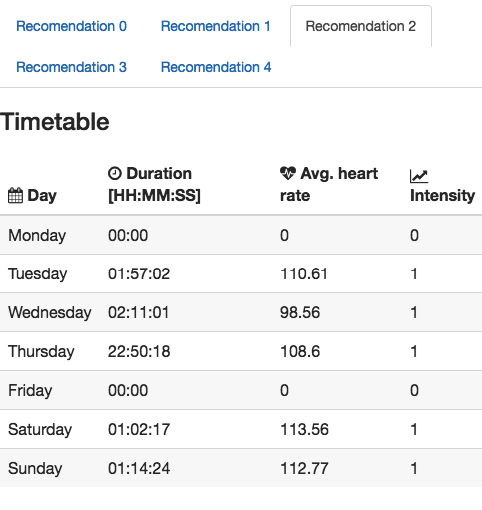
\includegraphics[width=\linewidth]{vizualization}
 \caption{Prikaz vizualizacije}
\end{figure}


\subsection{Rezultati}
V spodnjih tabelah so prikazani parametri za vsako metodo, pripadajoča natančnost in F1 metrika. 
\subsubsection{Metoda podpornih vektorjev}
Metoda se je najbolje obnesla z linearnim jedrom, najslabše pa z jedrom rbf. Parameter, ki omogoči krčenje na klasifikacijski model ni vplival. Prav tako v primeru jeder rbf in poly na model ni vplival parameter, ki omejuje maksimalno število iteracij, v primeru linearnega jedra pa se je omejevanje števila operacij izkazalo kot negativno.

 \small
 \setlength{\tabcolsep}{3pt}
 \begin{tabular}{|lrr|}
\hline
Metoda & Acc & F1 \\
\hline \hline
(kernel="rbf") & 77.35\% & 0.7532 \\
\hline
(kernel="rbf", max\_iter=50000) & 77.35\% & 0.7532 \\
\hline
(kernel="rbf", decision\_function\_shape="ovo") & 77.35\% & 0.7532 \\
\hline
(kernel="rbf", decision\_function\_shape="ovr") & 77.35\% & 0.7532 \\
\hline
(kernel="rbf", shrinking=False) & 77.35\% & 0.7532 \\
\hline
(kernel="poly") & 79.32\% & 0.7887 \\
\hline
(kernel="poly", max\_iter=50000) & 79.32\% & 0.7887 \\
\hline
(kernel="poly", decision\_function\_shape="ovo") & 79.32\% & 0.7887 \\
\hline
(kernel="poly", decision\_function\_shape="ovr") & 79.32\% & 0.7887 \\
\hline
(kernel="poly", shrinking=False) & 79.32\% & 0.7887 \\
\hline
(kernel="linear") & 79.53\% & 0.7913 \\
\hline
(kernel="linear", max\_iter=50000) & 78.60\% & 0.7816 \\
\hline
(kernel="linear", decision\_function\_shape="ovo") & 79.53\% & 0.7913 \\
\hline
(kernel="linear", decision\_function\_shape="ovr") & 79.53\% & 0.7913 \\
\hline
(kernel="linear", shrinking=False) & 79.53\% & 0.7913 \\
\hline
\end{tabular}

\normalsize

\subsubsection{Nevronske mreže}
Najboljši rezultat nevronskih mrež smo dobili pri uporabi aktivacijske funkcije tanh v kombinaciji z optimizacijsko metodo adam.
\begin{center}
 \small
 \setlength{\tabcolsep}{3pt}
 \begin{tabular}{|l r r|}
  \hline
  metoda & F1 & Accuracy \\
  \hline \hline
  adam-identity & 0.64 & 0.54\% \\
  \hline
  adam-logistic & 0.77 & 0.78\% \\
  \hline
  lbfgs-logistic & 0.69 & 0.70\% \\
  \hline
  lbfgs-tanh & 0.72 & 0.71\% \\
  \hline
  adam-relu & 0.71 & 0.69\% \\
  \hline
  lbfgs-relu & 0.63 & 0.60\% \\
  \hline
  lbfgs-identity & 0.61 & 0.52\% \\
  \hline
  adam-tanh & 0.79 & 0.80\% \\
  \hline
  sgd-identity & 0.00 & 0.49\% \\
  \hline
  sgd-tanh & 0.68 & 0.68\% \\
  \hline
  sgd-relu & 0.67 & 0.50\% \\
  \hline
  sgd-logistic & 0.00 & 0.49\% \\
  \hline
 \end{tabular}
\end{center}
\normalsize


\subsubsection{Odločitveno drevo}
Odločitveno drevo je vračalo podobne rezultate ne glede na nastavljene parametre. Rezultati pa so postajali slabši, če smo maksimalno globino zmanjšali pod 9.
\begin{center}
 \small
 \setlength{\tabcolsep}{3pt}
 \begin{tabular}{|l l l l r r|}
 \hline
  kriterij & vej. funk. & maks. globina & min. vej. & F1 & natančnost  \\
  \hline \hline
  gini & best & Brez & 2 & 0.7833 & 78.83\%  \\
  \hline
  entropy & best & Brez & 2 & 0.7841 & 78.88\%  \\
  \hline
  gini & random & Brez & 2 & 0.7834 & 78.77\%  \\
  \hline
  entropy & random & Brez & 2 & 0.7843 & 78.87\%  \\
  \hline
  gini & best & 9 & 5 & 0.7805 & 78.58\% \\
 \hline
\end{tabular}
\end{center}
\normalsize


\subsubsection{Ada Boost}
Pri ansambelski metodi število klasifikatorjev nad deset ni imelo velikega vpliva na natančnost.
\begin{center}
 \small
 \setlength{\tabcolsep}{3pt}
 \begin{tabular}{|l r r|}
 \hline
   št. klasifikatorjev & F1 & Natančnost \\
  \hline \hline
  10 & 0.7549 & 76.14\% \\
  \hline
  40 & 0.7876 & 79.19\% \\
  \hline
  70 & 0.7871 & 79.14\% \\
  \hline
  100 & 0.7873 & 79.16\% \\
  \hline
  130 & 0.7874 & 79.16\% \\
  \hline
 \end{tabular}
\end{center}
\normalsize


\section{Zaključek}
S tem eksperimentom smo želeli predlagati čim boljše treninge atletom, da bi imeli optimalen napredek.
Vsakega atleta smo najprej klasificirali in se probali naučiti kakšne treninge izvaja in pri tem ugotoviti kakšni treningi bi bili najbolj primerni za njega.
Pri tem smo uporabili odločitvena drevesa, metodo podpornih vektorjev in nevronske mreže.
Najboljše se je izkazala metoda [METODA], ki se z izbranimi, za naš problem optimalnimi parametri izkazala z [PROCENT] natančnostjo.
Zgradili smo tudi orodje za pregledovanje predlaganih treningov za naslednji teden, ki jih lahko uporabnik vidi preko brskalnika.
Potencialne izboljšave, ki bi lahko pripomogle k boljši klasifikaciji je ocena trenerja po vsakem treningu in počutje atleta med izvajanjem treninga, ki bi lahko imela velik vpliv na končni rezultat.

%
% The following two commands are all you need in the
% initial runs of your .tex file to
% produce the bibliography for the citations in your paper.
\bibliographystyle{abbrv}
\bibliography{mybib}  % mybib.bib is the name of the Bibliography in this case
% You must have a proper ".bib" file
%  and remember to run:
% latex bibtex latex latex
% to resolve all references
%
% ACM needs 'a single self-contained file'!
%

\balancecolumns
% That's all folks!
\end{document}
